\documentclass[12pt]{article}
\usepackage[utf8]{inputenc}
\usepackage{amsmath}
\usepackage{graphicx}
\usepackage[ruled, vlined]{algorithm2e}
\usepackage{algpseudocode}
\usepackage{listings}
\usepackage{color}
\usepackage{caption}
\usepackage{subcaption}

\graphicspath{ {./images/} }

\definecolor{dkgreen}{rgb}{0,0.6,0}
\definecolor{gray}{rgb}{0.5,0.5,0.5}
\definecolor{mauve}{rgb}{0.58,0,0.82}

\lstset{language=Python,
  aboveskip=3mm,
  belowskip=3mm,
  showstringspaces=false,
  columns=flexible,
  basicstyle={\small\ttfamily},
  numbers=none,
  numberstyle=\tiny\color{gray},
  keywordstyle=\color{blue},
  commentstyle=\color{dkgreen},
  stringstyle=\color{mauve},
  breaklines=true,
  breakatwhitespace=true,
  tabsize=3
}

\title{On Synchronization Algorithms for the Optimization of Resources in Agriculture}
\author{Leonardo D. Garcia}
\date{\today}

\begin{document}

\maketitle

\begin{abstract}
This report examines a systems-based approach on the synchronization and optimization of resources in the agriculture sector. By providing an algorithmic aspect inspired by the dining philosophers problem from operating systems theory, it is possible to generate a concurrent program that will simulate the system dynamics of the plant models considering the sharing of limited resources such as water.
\end{abstract}

\small
\textbf{\textit{Keywords:}} multithreading, irrigation, algorithm, resources.

\section{Objectives}
The objectives of this paper focus on the capability of the present individual to formalize a contemporary viewpoint into the techniques that can be used in control engineering for the regulation and stability of dynamical systems. \\

Operating systems are the software pillars that holds together the organized aspects of the computer architecture. Although a computer by itself can work properly, the operating system controls and coordinates the management of physical resources inside the machine to provide the swiftest and best regulated of computing procedures. \\

Given the accelerated abilities of the processors, it has been proposed that one can employ the very same algorithms that the OS utilizes for their handling of shared data and memory locations in a similar way that generates an analogy to the inputs to withhold the stability of a plant—an irrigation area that must share its water with other adjacent sectors. \\

In essence, the purpose of this experiment is in the adaptation of a concurrent, synchronization algorithm from operating systems theory into a simple yet elegant solution that can be used for the reservation of input energy. \\

\section{Theoretical Framework}

\subsection{Irrigation Areas}

An irrigation area is a finite-sized polygonal space where crops are grown throughout the year’s seasons. Like other real functional systems, they can be modeled mathematically as a linear-time invariant (LTI) system. A disadvantage in trying to do so lies on the fact that real systems usually present nonlinearities which complicate their analysis. \\

An alternative to preserve the advantages and strengths of an LTI system is by linearizing the plant on different operating points. As a result, a piecewise model of the plant is generated. \\

For this LTI models, a state-space approach is taken instead of a transfer function model to consider the controllability and observability of the plant for a MIMO model \cite{ogata}. The state equations for these cases are presented in Equations \ref{eqn:1} \& \ref{eqn:2}.

\begin{equation}
\label{eqn:1}
\mathbf{\dot{x}}(t) = \mathbf{A x}(t) + \mathbf{B u}(t)
\end{equation}
\begin{equation}
\label{eqn:2}
\mathbf{y}(t) = \mathbf{C x}(t) + \mathbf{D u}(t)
\end{equation}

$\mathbf{A}$ is the state matrix, $\mathbf{B}$ is the input matrix, $\mathbf{C}$ is the output matrix, and $\mathbf{D}$ is the transmission matrix. To avoid any major complication with the study of the irrigation areas, second-order models were identified from each of four distinct areas in previous studies from Dr. Camilo Lozoya. \\

These models depend thus on two state variables and two input variables. The state variables are the soil moisture $\theta(t)$ and the rate of change of the moisture with respect to time $\dot{\theta}(t)$. The input variables are from the other hand the irrigation level $ir(t)$ and the evapotranspiration (ETO) of the soil. The ETO is modified by a proportional parameter called $K_c$, which is denominated the crop constant and is a dimensional constant to regulate every area \cite{camilo2}. These changes from area to area. \\

In the end, the vector expressions for these variables are displayed in Equations \ref{eqn:3} \& \ref{eqn:4}.

\begin{equation}
\label{eqn:3}
\mathbf{x}(t) = 
\begin{bmatrix}
\theta(t) & \dot{\theta}(t)
\end{bmatrix}
^T
\end{equation}
\begin{equation}
\label{eqn:4}
\mathbf{u}(t) = 
\begin{bmatrix}
ir(t) & K_c ETO(t)
\end{bmatrix}
^T
\end{equation}

The actual state equations must be separated according to three levels. The denominated previous investigations from Dr. Lozoya categorize the advancements of water consumption unto two thresholds \cite{camilo1}. The first threshold separates what is considered the gravitational water, which is the excess water that remains after an irrigation cycle. It can be found at the top of the moisture level diagram. \\

The next phase is the stable region, which is the most preferrable because it keeps in place the safety of the plant. No hazardous risks relating to water shortage occur at this point. There is a middle bias line that represents the most optimal operating point for the area. This specific offset depends on the irrigation area and most of the times can only be estimated experimentally. \\

Hydric stress then becomes an urgent problem once the plant leaves the stable region. It is at this point where the lack of water becomes significative to the vegetation and therefore can spawn visible damage sooner or later pertaining to the drought of the crop region. Fig. \ref{fig:1} depicts a crude diagram of these operating zones for a sample model. \\

\begin{figure}[h]
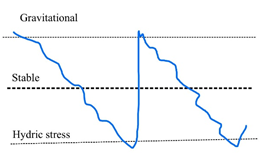
\includegraphics{dynamics}
\label{fig:1}
\centering
\caption{Levels of soil moisture for the plant.}
\end{figure}

In total, three state matrices and three input matrices were formed depending on the level of water consumption present \cite{camilo3}. These are presented as Equations \ref{eqn:5} to \ref{eqn:10} here below. \\

\begin{equation}
\label{eqn:5}
\mathbf{A}_{above}(t) = 
\begin{bmatrix}
0.98501 & 0.00001 \\
0.00001 & 0.98501
\end{bmatrix}
\end{equation}

\begin{equation}
\label{eqn:6}
\mathbf{A}_{middle}(t) = 
\begin{bmatrix}
1.00000 & 0.00001 \\
0.00001 & 0.98501
\end{bmatrix}
\end{equation}

\begin{equation}
\label{eqn:7}
\mathbf{A}_{below}(t) = 
\begin{bmatrix}
1.00000 & 0.00001 \\
0.00001 & 0.98501
\end{bmatrix}
\end{equation}

\begin{equation}
\label{eqn:8}
\mathbf{B}_{above}(t) = 
\begin{bmatrix}
0.00245 & -0.00004 \\
0.00300 & -0.00020
\end{bmatrix}
\end{equation}

\begin{equation}
\label{eqn:9}
\mathbf{B}_{middle}(t) = 
\begin{bmatrix}
0.00135 & -0.00060 \\
0.00325 & -0.00050
\end{bmatrix}
\end{equation}

\begin{equation}
\label{eqn:10}
\mathbf{B}_{below}(t) = 
\begin{bmatrix}
0.00125 & -0.00005 \\
0.00150 & -0.00035
\end{bmatrix}
\end{equation}

\subsection{Multithreading}

A process thread is a unit of processor utilization that permits the running of a set of operations within the core of the computer. Modern computers permit the capability of running multiple threads in a single processor. This allows the event of running various processes simultaneously. \\

While this seems to propose the opportunity to run processes in parallel, it does not work like that. Threads are concurrent: they each advance step by step waiting for the others to continue. Because they interrupt each other little by little at the high frequencies of the computer clock, it can be felt that they operate asynchronously. \\

The act of running different threads in a single core to apparent a parallel process is called multithreading. Because they do not work in parallel, frequently problems arise relating to the synchronization of resources, where threads may quarrel between each other of the utilization of one. Another problem can be if the threads wait each other to finish, creating a cycle that will never end. This event is termed a deadlock in computer science. \\

\subsubsection{Dining Philosophers Problem}

To solve the problem, a mind experiment was performed by computer scientists Edsger W. Dijkstra and Tony Hoare back in the 1960s. Let there be \emph{n} philosophers seated in a round table. Before them come plates of noodles, each for each philosopher \cite{osbook}. Fig. \ref{fig:2} exemplifies this. \\

\begin{figure}[h]
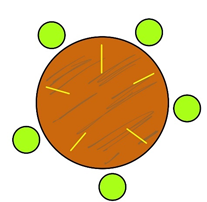
\includegraphics{phil}
\label{fig:2}
\centering
\caption{Dining philosophers table.}
\end{figure}

To eat their noodles, they must use a pair of chopsticks. Nonetheless, they find a problem: everyone must share at least one chopstick with their adjacent neighbor. Therefore, one’s right neighbor shares their left chopstick, and the parallel with the left neighbor. Because one must use the whole pair to be able to eat, there comes the question: who eats? \\

The solution is very simple, although it sounds complex to implement whoever reaches the chopsticks first gets to eat first. All others who did not reach them must wait for the others to eat, hoping not to starve while waiting. When those who are eating finish, they leave the chopsticks back in the table, and let others (whoever reaches them first) to eat. To implement it in code, one must use a concept called a mutex. \\

A mutex is an abstract object that can be blocked so that if other threads attempt to grab them, they are unable and must wait for the process to release the mutex. Hence, they permit the synchronization of concurrent processes without the fear of robbing the resources at an inappropriate moment. \\

The operation to collect the mutexes if available is called \emph{wait}, because one waits for them to be free. To release them, one simply \emph{signals} the computer that they are free once again. The algorithm, short and easy, is shown below. \\

\begin{algorithm}[H]
\SetAlgoLined
\While{True}{
\textbf{wait} chopstick[\textit{i}]\;
\textbf{wait} chopstick[(\textit{i}+1) \% \textit{n}]\;
... \hfill\\
/* eating */\\
... \hfill\\
\textbf{signal} chopstick[\textit{i}]\;
\textbf{signal} chopstick[(\textit{i}+1) \% \textit{n}]\;
... \hfill\\
/* thinking */\\
... \hfill\\
}
\caption{Dining philosophers problem}
\end{algorithm}

\section{Experiment}

\subsection{Program Description}

The program can therefore be passed to a real computer language where the practical aspects of coding in the real world are put to the test. The language picked for the task was Python, because it is a very simple yet useful language with a broad range of available libraries for things like numeric operations and multithreading. \\

As a first job, it is important to define the object to simulate. It is proposed that the irrigation area be defined as a class, where one group several instances to recreate the adjacent groups of irrigation areas. This class must possess various attributes, including the crop constant and threshold levels for simulation. \\

The methods recommended for the class (besides the constructor) include irrigation dynamics function that returns the next state for the plant according to the input variables and the previous states of the system. According to the soil moisture level, the state equation can take one of the many forms planted in Equations 5 to 10. \\

When running the simulation, the control action depends on the region where the humidity finds itself, and whether other resources are available. Because all irrigation areas use the same water, this water source will be blocked as a mutex. As a result, when one is in the hydric stress region, it can only be watered if no other area is under irrigation. When it reaches the gravitational water region, it releases the mutex for the rest of the areas to fight for them. \\

Section \ref{code:1} presents a view into the Python script, including documentation and comments that serve as explanatory aid for the reader. \\

\subsection{Python Code}
\label{code:1}

\begin{lstlisting}

import numpy as np
import matplotlib.pyplot as plt
from scipy.io import loadmat

class AreaSimulation:

    def __init__(self, xk_initial, Kc, control_high, control_low, irrigation_value):
        self.xk_initial = xk_initial
        self.xk_array = np.empty(0)
        self.ir_array = np.empty(0)
        self.Kc = Kc
        self.control_high = control_high
        self.control_low = control_low
        self.irrigation_value = irrigation_value
        self.eto_array = np.empty(0)
        self.t_array = np.empty(0)

    def irrigation_dynamics_function(self, xk_initial, ir_act, eto_act, Kc):

        A_above = np.array([[0.98501, 0.00001], [0.00001, 0.98501]])
        A_middle = np.array([[1.00000, 0.00001], [0.00001, 0.98501]])
        A_below = np.array([[1.00000, 0.00001], [0.00001, 0.98501]])

        B_above = np.array([[0.00245, -0.00004], [0.00300, -0.00020]])
        B_middle = np.array([[0.00135, -0.00060], [0.00325, -0.00050]])
        B_below = np.array([[0.00125, -0.00005], [0.00150, -0.00035]])

        C = np.array([1, 0])

        high_limit = 7.0
        low_limit = -7.0
        high_threshold = 5.0
        low_threshold = -5.0

        xk_act = xk_initial
        uk_act = np.array([ir_act, Kc*eto_act], dtype=object)

        xk_next = np.empty(2)

        if xk_act[0] > high_threshold:
            xk_next = np.dot(A_above, xk_act) + np.dot(B_above, uk_act)
        elif xk_act[0] > low_threshold:
            xk_next = np.dot(A_middle, xk_act) + np.dot(B_middle, uk_act)
        else:
            xk_next = np.dot(A_below, xk_act) + np.dot(B_below, uk_act)
            
        if xk_next[0] > high_limit:
            xk_next[0] = high_limit
        elif xk_next[0] < low_limit:
            xk_next[0] = low_limit

        return xk_next
    
    def run(self, filename):
        data = loadmat(filename)
        self.eto_array = data['eto_array']
        
        simulation_period = self.eto_array.size
        self.t_array = np.arange(simulation_period)
        
        self.xk_array = np.empty([2, simulation_period])
        self.ir_array = np.empty([simulation_period])
        self.ir_array[0] = 0.0
        
        for t in range(simulation_period):
            xk_next = self.irrigation_dynamics_function(self.xk_initial, self.ir_array[t], self.eto_array[t], self.Kc)
            self.xk_initial = xk_next
            self.xk_array[0, t] = xk_next[0]
            self.xk_array[1, t] = xk_next[1]
            
            if t == simulation_period-1:
                break
            
            if xk_next[0] > self.control_high:
                self.ir_array[t+1] = 0.0
            elif xk_next[0] < self.control_low:
                self.ir_array[t+1] = self.irrigation_value
            else:
                self.ir_array[t+1] = self.ir_array[t]
    
    def display(self, title):
        simulation_period = self.eto_array.size
        
        plt.title(title)
        plt.plot(self.t_array, self.xk_array[0], 'b-', 
                 self.t_array, np.zeros(simulation_period), 'k--',
                 self.t_array, self.control_high*np.ones(simulation_period), 'k:',
                 self.t_array, self.control_low*np.ones(simulation_period), 'k:')
        plt.axis([0, simulation_period, -8, 8])
        
        plt.show()



if __name__ == "__main__":
    Areas = [None]*4

    xk_initial = [np.array([5.0, 0.0]), np.array([2.0, 0.0]),
                np.array([2.0, 0.0]), np.array([-2.0, 0.0])]
    Kc = [1.0, 1.2, 1.4, 0.8]
    control_high = [5.0, 1.0, 2.0, 4.0]
    control_low = [-5.0, -1.0, -2.0, -4.0]
    irrigation_value = [40.0, 45.0, 35.0, 40.0]

    filename = r"C:\Users\leodg\Documents\TecMTY\Sem_9\Research Internship\notebook\DataSet_ETO_45_days.mat"

    for i in range(len(Areas)):
        Areas[i] = AreaSimulation(xk_initial=xk_initial[i], Kc=Kc[i],
                            control_high=control_high[i], control_low=control_low[i],
                            irrigation_value=irrigation_value[i])
        Areas[i].run(filename)
        Areas[i].display(f"Area {i+1}")

\end{lstlisting}


\section{Results}

After running the simulation, the following four charts (Fig. \ref{fig:3}) were delivered by the program. They are for the four areas defined in lines 246 to 268 of the script. Fig. \ref{fig:3a} \& \ref{fig:3d} do not seem off by any means. The swift changes that do look visible in plain eye are in Fig. \ref{fig:3b} \& \ref{fig:3c}. \\

There are some huge notches where the plants are under some harsh hydric stress states. The reason for this is because, as water becomes utilized by any other plant, they must wait for the resource to be liberated in order to replenish. Additionally, because the areas do not follow any priority queue, it is a tournament to see who reaches first the water. \\

What the experiment helped demonstrate is that these operating system concepts can be employed in any other area, and one must seize these algorithms to create an opportunity of optimization and synchronization in the daily aspects of the industrial life. \\

\begin{figure}[h]
\label{fig:3}
\centering

\begin{subfigure}[b]{0.475\textwidth}
\label{fig:3a}
\centering
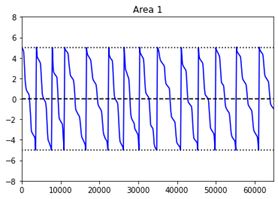
\includegraphics[width=\textwidth]{area1}
\caption{Area 1.}
\end{subfigure}
\hfill
\begin{subfigure}[b]{0.475\textwidth}
\label{fig:3b}
\centering
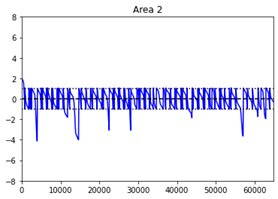
\includegraphics[width=\textwidth]{area2}
\caption{Area 2.}
\end{subfigure}
\vskip\baselineskip
\begin{subfigure}[b]{0.475\textwidth}
\label{fig:3c}
\centering
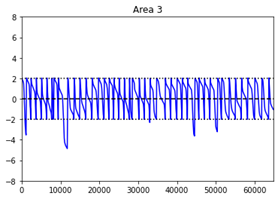
\includegraphics[width=\textwidth]{area3}
\caption{Area 3.}
\end{subfigure}
\hfill
\begin{subfigure}[b]{0.475\textwidth}
\label{fig:3d}
\centering
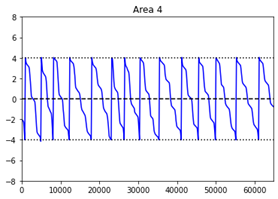
\includegraphics[width=\textwidth]{area4}
\caption{Area 4.}
\end{subfigure}

\caption{Irrigation Areas Simulation.}
\end{figure}

\section{Conclusions}

To conclude, the experiment can be considered a huge success in term of adapting a simulation model for a real system that can make use of synchronization techniques of computer science for the applications of automatic control engineering. \\

The next step in this arduous scientific process delves into the formalization of the experiment using a real-time embedded system architecture in an actual irrigation area. This will help to solidify the validity of the algorithm and discover any other perturbance that may be affecting the plant. \\

\bibliographystyle{ieeetr}
\bibliography{references}

\end{document}
